\documentclass[11pt,a4paper]{article}
\usepackage[margin=0.95in]{geometry}
\usepackage{times}
\usepackage{amsmath,amssymb}
\usepackage{graphicx}
\usepackage{booktabs}
\usepackage{enumitem}
\usepackage{titlesec}
\usepackage{xcolor}
\usepackage{fancyhdr}
\usepackage{caption}
\usepackage[colorlinks=true,linkcolor=black,citecolor=blue,urlcolor=blue]{hyperref}
\graphicspath{{../../results/figures/}}
\titleformat{\section}{\large\bfseries}{\thesection}{1em}{}
\titleformat{\subsection}{\normalsize\bfseries}{\thesubsection}{1em}{}
\titlespacing*{\section}{0pt}{12pt}{5pt}
\titlespacing*{\subsection}{0pt}{9pt}{3pt}
\setlist[itemize]{topsep=2pt,itemsep=1pt,parsep=0pt}
\setlist[enumerate]{topsep=2pt,itemsep=1pt,parsep=0pt}
\captionsetup{font=small,labelfont=bf}
\pagestyle{fancy}\fancyhf{}
\fancyhead[L]{\small Seeing Through the Shake --- Final Report}
\fancyhead[R]{\small\thepage}
\renewcommand{\headrulewidth}{0.4pt}

\title{\bfseries Seeing Through the Shake: Text-Aware PSF Estimation\\for Blind Motion Deblurring of License Plates and Low-Texture Text\\[6pt]\large Final Report --- Digital Image Processing}
\author{Inesh Roy (2024112015) \and Maithily Gauravkumar Bhala (2024117011)}
\date{}

\begin{document}
\maketitle
\thispagestyle{fancy}

\begin{abstract}
Classical blind motion deblurring reads the blur angle and length off the image's own spectrum
(Radon transform and cepstrum) and inverts it with Richardson--Lucy deconvolution. It needs no
training data and is fully interpretable, but it is developed on texture-rich photographs. We
study it on license plates and printed text, add a text-aware stage and a confidence gate, and
evaluate the complete pipeline on synthetic blur, the K\"ohler camera-shake benchmark and two public
datasets of real blurred plates. A controlled sweep (8 angles $\times$ 5 lengths $\times$ 4 noise
levels) shows that text content is not what breaks the estimator --- printed text in a plate-sized
window is its easiest input (98.9\% success) --- but region size, noise and short blurs are. The
planned edge-enhancing pre-processing \emph{halves} estimation success; what strengthens the blur
signature on real plates is the opposite operation, restricting the search to the low band where
resampled, compressed plate crops still carry signal. The final multi-band estimator raises OCR
character accuracy on 397 held-out real motion-blurred plates (LPBlur) from 0.18 (blurred) and
0.24 (classical baseline) to 0.50. A gate that requires a deep cepstral dip and agreement between
image halves refuses 96--100\% of the harmful restorations on held-out synthetic data and on
LPBlur makes only 0.8\% of the plates worse, while keeping a 2.3$\times$ accuracy gain. On
CCPD-Blur, where the blur is mostly not linear motion, it refuses 82\% of the images and recovers
most of the damage that unconditional deblurring causes, but does not improve on leaving those
images alone.

\end{abstract}

% ================= INTRODUCTION =================
\section{Introduction}

Classical blind motion deblurring recovers a sharp image without knowing the blur kernel by
reading the kernel off the blurred image's own spectrum: the angle of a linear motion blur from a
Radon transform of the log-spectrum and its length from the cepstrum, followed by non-blind
deconvolution such as Richardson--Lucy~\cite{richardson1972,lucy1974,cannon1976,moghaddam2007,oliveira2007}.
The approach needs no training data and every intermediate quantity can be inspected, but it was
developed and is nearly always evaluated on texture-rich natural photographs.

License plates and printed text are a different kind of input: small, low-contrast, dominated by a
few straight strokes and, in practice, resampled and compressed. Our proposal hypothesised that the
classical estimator is weakest exactly there, planned a text-contrast pre-processing stage to
strengthen the blur signature, and a confidence gate so that an untrustworthy estimate is refused
instead of silently making the image worse.

This report describes the full system and an evaluation that follows the proposal's five
objectives: (O1) the core pipeline validated against known kernels on synthetic blur and on the
K\"ohler camera-shake benchmark~\cite{kohler2012}; (O2) a controlled angle $\times$ length $\times$
noise sweep quantifying where it fails on natural images (Kodak) versus text and plates;
(O3) the pre-processing stage measured on the same sweep; (O4) the gate's trade-off between
harm avoided and good restorations withheld; and (O5) the full pipeline on real blurred plates from
public datasets (LPBlur~\cite{lpblur2024} and CCPD-Blur~\cite{ccpd2018}), with OCR accuracy before
and after restoration against the classical baseline.

\paragraph{Summary of findings.}
\begin{enumerate}
  \item \textbf{The difficulty is region size, noise and short blur, not text content.}
        In a plate-sized window printed text is the estimator's easiest input (98.9\% success),
        plates reach 89.4\% and natural texture 80.7\%; the same natural images reach 93.0\% at full
        frame. The gap the proposal expected is a \emph{small-region} gap --- exactly where plates
        live --- concentrated on short blurs under noise.
  \item \textbf{Edge enhancement does not strengthen the signature; band limiting does.} The planned
        edge-enhanced, locally normalised input halves estimation success (46.5\% vs.\ 89.7\%), and
        derivative operators in general collapse under noise; only a mild Gaussian high-pass helps on
        synthetic data (+2.5 points). On real plates the decisive operation is the opposite one:
        discarding the upper spectrum, where resampling and compression residue hide the nulls. The
        final text-aware stage is a multi-band search, which raises OCR accuracy on held-out real
        motion-blurred plates from 0.18 (blurred) and 0.24 (classical baseline) to 0.50.
  \item \textbf{The gate makes the pipeline safe to run.} Requiring a deep dip and agreement between
        image halves, it refuses 96--100\% of harmful restorations on held-out synthetic data; on
        LPBlur only 0.8\% of plates get worse. On CCPD-Blur, whose blur is mostly not linear motion,
        unconditional deblurring cuts accuracy from 0.76 to 0.19; the gate refuses 82\% of the
        images and recovers most of the loss (0.68), though it does not beat leaving them alone.
  \item \textbf{A correction to phase 0.} The Radon-variance angle is a more robust cue than an
        unrestricted joint (direction $\times$ lag) search; the final estimator uses the Radon angle
        with a $\pm3^\circ$ joint refinement, i.e.\ the proposal's pipeline as written.
\end{enumerate}
All numbers in this report are regenerated by \texttt{experiments/run\_all.py}; design choices were
made on development splits disjoint from every reported test image.

% ================= METHOD =================
\section{Method}
\label{sec:method}

\subsection{Blur model}
A uniform motion blur is modelled as $b = l * k + n$, where $l$ is the sharp image, $n$ is
noise and $k$ is a line kernel of length $L$ pixels at angle $\theta$ (counter-clockwise from
the $x$ axis). We generate $k$ by area sampling of the line segment, so non-integer lengths
and arbitrary angles are exact up to discretisation and an axis-aligned kernel is an exact box.
In the frequency domain $B = L\cdot K + N$ with
\begin{equation}
  |K(\omega)| = \left|\operatorname{sinc}\!\left(L\,\langle\omega, u_\theta\rangle\right)\right|,
\end{equation}
which vanishes on parallel lines perpendicular to the motion direction $u_\theta$, spaced
$1/L$ cycles per pixel apart. Both blur parameters are encoded in this null pattern: its
orientation gives $\theta$ and its spacing gives $L$.

\subsection{Radon--cepstrum estimator}
The estimator works on the log-magnitude spectrum $S = \log(\epsilon + |\mathcal{F}\{w\cdot g\}|)$
of the windowed (Tukey), mean-removed grayscale image $g$, zero-padded to a square grid of at
least $256\times256$ so that all directions are sampled isotropically. The spectrum is median
centred and multiplied by a raised-cosine disc that ends at a radial band limit $c$ (a fraction
of Nyquist; $c=1$ uses the full band).

\paragraph{Radon transform.} The Radon transform $R_\phi(s)$ of $S$ integrates the spectrum along
lines at angle $\phi$. Along the direction of the null stripes the integration lines follow the
stripes, so the projection perpendicular to them oscillates with period $1/L$.
We compute it by rotating the spectrum and summing columns (verified to match
\texttt{skimage.transform.radon} to numerical precision and $\sim$10$\times$ faster),
for $\phi = 0,1,\dots,179^\circ$.

\paragraph{Cepstrum along each projection.} The 1-D Fourier transform of each projection is,
by the projection--slice theorem, a radial slice of the 2-D cepstrum
$C = \mathcal{F}^{-1}\{\log|B|\}$ (verified numerically in the test suite). For a box blur of
length $L$, $\log|\operatorname{sinc}|$ has period $1/L$ and its cepstrum has a strong
\emph{negative} peak at lag $L$. The (direction, lag) map
$P(\phi, q)$ therefore shows a single deep negative dip at $(\theta, L)$.

\paragraph{Angle, then length.} The Radon angle $\theta_R$ is the direction of maximum variance
of the projections of $S$ (DC masked, short rim chords ignored): integrating along the null
stripes keeps them separate, so that projection oscillates the most. The length is the lag of the
deepest negative dip of $P(\theta, q)$ for $q\in[q_{\min}, q_{\max}]$, refined by parabolic
interpolation. Our estimator searches $P$ jointly over $q$ and the directions within
$\pm3^\circ$ of $\theta_R$, then refines the angle at $0.25^\circ$ resolution, so a slightly
misplaced variance maximum is corrected by the cepstral evidence.

Phase~0 had suggested replacing the Radon angle by an unrestricted joint search over all
directions, on the grounds that strong strokes compete with the blur stripes in the variance. The
full evaluation showed the opposite: the unrestricted search is fooled by isolated deep dips in
the wrong direction more often than the variance rule is fooled by strokes. On the development
split the windowed refinement beat both alternatives (90.7\% success, vs.\ 89.5\% for the textbook
two-stage rule and 85.5\% for the unrestricted search; mean angle error $1.3^\circ$ vs.\
$1.4^\circ$ and $5.5^\circ$). This was noticed when the first test-split sweep ranked the
two-stage rule above the unrestricted search; the choice itself was then made on development data
only, and both alternatives are reported as reference rows.

\subsection{The text-aware stage}
\label{sec:textaware}
The proposal planned a text-contrast pre-processing step (local contrast normalisation and
edge enhancement) in front of the estimator. We implemented and evaluated nine such operators
(CLAHE, unsharp masking, Gaussian high-pass, Laplacian, difference of Gaussians, gradient
magnitude, local contrast normalisation, homomorphic filtering, and the proposed
LCN+Laplacian combination) on the identical sweep (Section~\ref{sec:preproc}). Contrast
normalisation was neutral, the derivative operators --- including the proposed combination ---
collapsed under noise because they raise exactly the high-frequency band where noise, JPEG residue
and resampling artefacts live and where the blur nulls are weakest, and only a mild Gaussian
high-pass helped on synthetic data. On real plates none of the contrast operators moved OCR
accuracy (Section~\ref{sec:design}).

The analysis pointed the other way. Plates and printed text in real photographs are small,
resampled and compressed regions, so the upper part of their spectrum carries little genuine
signal. The final text-aware stage is therefore a \emph{band-limited multi-band search}: the joint
search is run three times with band limits $c\in\{1, 0.5, 0.3\}$ and the estimate whose dip is
most \emph{directional} (largest $z_\angle$, below) is kept. Long blurs, whose nulls are densely
spaced at low frequencies, are then found in the clean low band; short blurs, whose first null
lies beyond $0.3$ Nyquist, are still found in the full band. The configuration was chosen on
development data only (Section~\ref{sec:design}).

\subsection{Confidence gate}
\label{sec:gate}
Deconvolution with a wrong kernel does not merely fail to sharpen: it amplifies the wrong
frequencies and leaves ringing and ghost strokes that make the plate \emph{less} legible. The gate
turns that silent failure into an explicit refusal (``not confident --- image returned
unchanged''). It combines three tests, each computed from quantities the estimator already has:
\begin{itemize}
  \item \textbf{Dip depth} (\emph{confidence}): depth of the winning dip against the background of
        the whole (direction, lag) map, in robust standard deviations (median/MAD).
  \item \textbf{Directional contrast} $z_\angle$: depth of the winning dip against the
        \emph{other directions at the same lag}. A linear-motion dip exists in one direction
        only, whereas isotropic structure --- defocus, soft or band-limited content, noise
        texture --- is deep in every direction and scores near zero.
  \item \textbf{Split-half agreement}: a uniform blur is the same everywhere, so the estimate is
        repeated on the left, right, top and bottom halves of the region; the number of halves
        (0--4) that reproduce the angle (within $10^\circ$) and length (within
        $\max(2\,\text{px}, 15\%)$) is counted.
\end{itemize}
A threshold of 0 switches a test off. The thresholds are calibrated on development data
(Section~\ref{sec:gateexp}); the resulting gate uses dip depth and split-half agreement.

\subsection{Non-blind restoration}
Richardson--Lucy (RL) is the primary restorer. Real images are not periodic and content outside
the frame is unknown, so we use the masked (unknown-boundary) RL variant: the estimate lives on a
canvas padded by the kernel radius and the data term is evaluated only on the observed pixels,
which removes the boundary ringing that periodic RL produces. For the synthetic sweeps, iterations
are stopped by the discrepancy principle (residual variance reaching the noise variance estimated
from the finest diagonal Haar detail band with the Donoho--Johnstone MAD estimator), because the best iteration count
depends strongly on noise (Section~\ref{sec:truepsf}). On real plates we use a fixed 30 iterations
as in the proposal. Wiener deconvolution with an edge-tapered canvas is implemented as the
comparison method.

\subsection{Evaluation-only OCR}
Legibility is measured with an off-the-shelf recogniser (RapidOCR, recognition model only) applied
to the plate after perspective rectification with the dataset's corner annotations. It is a
measuring instrument and never part of the restoration. Chinese plates start with a province
glyph; we score the six alphanumeric characters (character accuracy $=1-$ edit distance$/6$).
On sharp CCPD plates the instrument reads 100\% of the characters correctly.

% ================= EXPERIMENTS =================
\section{Experiments}
\label{sec:experiments}

\subsection{O1: restoration with a known kernel}
\label{sec:truepsf}
Before estimating anything, the non-blind step was checked with the \emph{true} PSF on the
development sources (1{,}440 trials over lengths, angles and noise levels; Fig.~\ref{fig:truepsf}).

\begin{figure}[h]
\centering
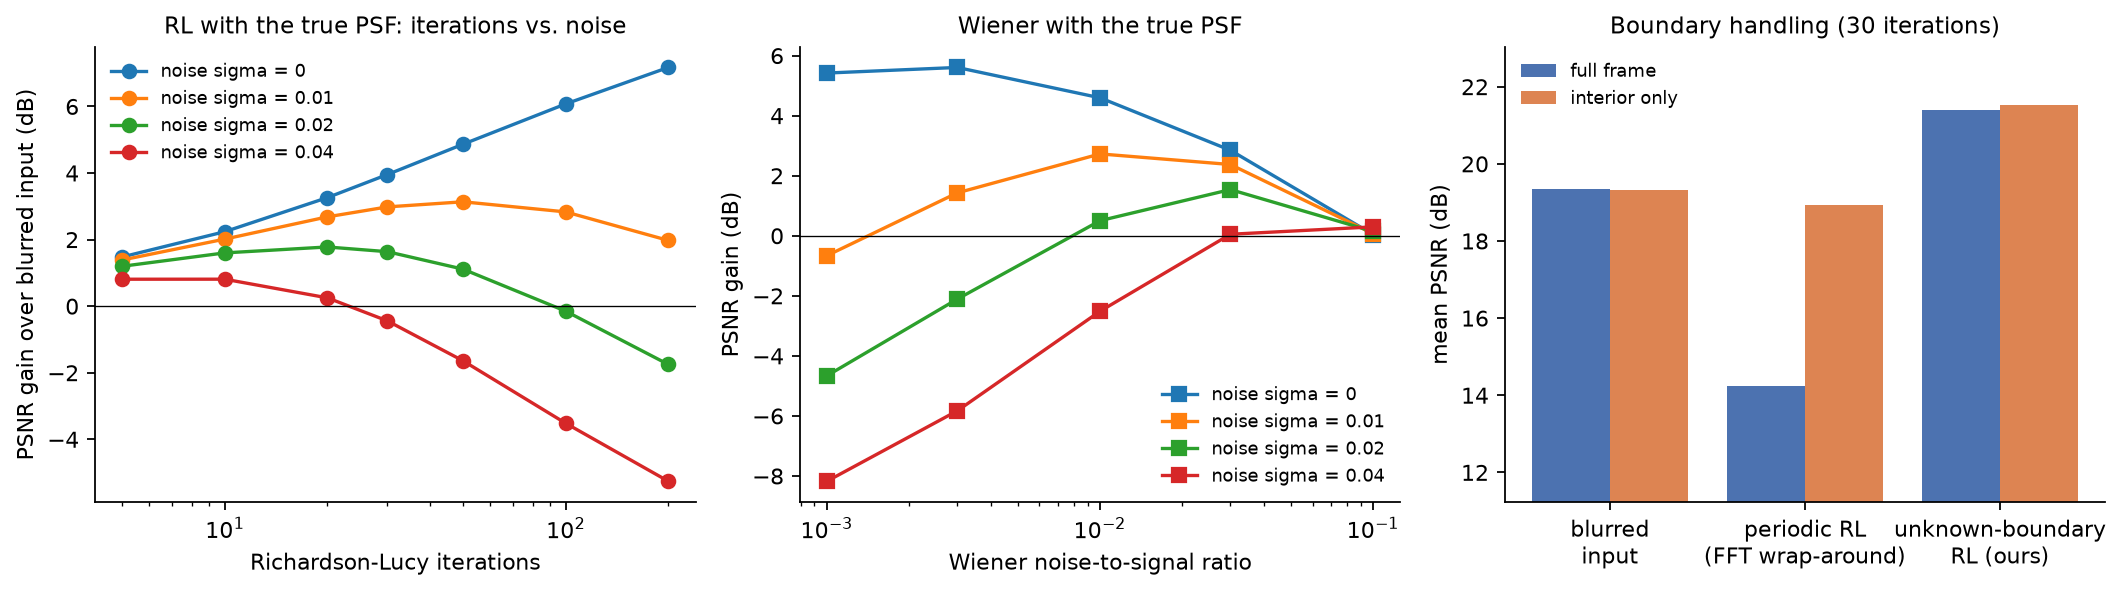
\includegraphics[width=\textwidth]{01_true_psf.png}
\caption{Restoration with the true PSF. Left: RL gain vs.\ iterations for four noise levels.
Middle: Wiener gain vs.\ noise-to-signal ratio. Right: boundary handling at 30 RL iterations.}
\label{fig:truepsf}
\end{figure}

\begin{itemize}
  \item \textbf{RL iterations depend on noise.} Without noise the gain keeps growing (+7.2\,dB at
        200 iterations); at $\sigma=0.04$ it peaks at about 10 iterations and becomes negative
        beyond 20, because RL then fits the noise. Stopping by the discrepancy principle (residual
        reaches the estimated noise level, $\tau=1$) gives a positive gain at every noise level:
        $+4.8$, $+2.3$, $+1.5$ and $+0.7$\,dB at $\sigma = 0, 0.01, 0.02, 0.04$. All synthetic
        restorations use this rule.
  \item \textbf{Boundaries matter.} Periodic RL wraps the image around, and the ringing this
        causes at the borders drops full-frame PSNR from 19.4\,dB (blurred) to 14.2\,dB.
        Unknown-boundary RL reaches 21.4\,dB on the full frame and 21.5\,dB in the interior.
  \item \textbf{Wiener} needs its noise-to-signal ratio matched to the noise level (best NSR
        moves from $0.003$ to $0.1$ as $\sigma$ grows); a mismatched NSR loses up to 8\,dB.
\end{itemize}

\subsection{Design choices on development data}
\label{sec:design}
All configuration choices were made on development data that no reported number uses: the
synthetic dev split (8 sources per class, the full grid: 3{,}840 trials per variant) and dev
subsets of LPBlur (147 usable pairs) and CCPD-Blur (150 images), scored by OCR accuracy after RL with
each variant's estimate (\texttt{experiments/00\_design\_dev.py}). Table~\ref{tab:design}
summarises the evidence for the text-aware stage.

\begin{table}[h]
\centering\small
\begin{tabular}{lccc}
\toprule
variant (in front of the baseline estimator) & synthetic success & LPBlur OCR & CCPD-Blur OCR \\
\midrule
blurred input, no restoration & -- & 0.234 & 0.768 \\
plain grayscale (baseline) & 90.7\% & 0.280 & 0.256 \\
CLAHE & 87.8\% & 0.280 & 0.234 \\
local contrast normalisation & 91.4\% & 0.289 & 0.339 \\
homomorphic filtering & 90.5\% & 0.253 & 0.274 \\
LCN + Laplacian (proposed edge-enhanced stage) & 46.4\% & 0.239 & 0.584$^\ast$ \\
SNR-adaptive band limit & 79.7\% & 0.332 & 0.171 \\
band limit 0.5 Nyquist & 75.1\% & 0.463 & 0.137 \\
band limit 0.3 Nyquist & 55.4\% & \textbf{0.637} & 0.098 \\
\textbf{multi-band search} $\{1, 0.5, 0.3\}$ (final) & 87.6\% & 0.515 & 0.214 \\
\bottomrule
\end{tabular}
\caption{Development evidence. $^\ast$Scores well only because it returns very short kernels
(median 8\,px) that barely change the image; it is the worst variant at estimating blur.}
\label{tab:design}
\end{table}

Two observations decided the design. First, contrast operators do not move real-plate accuracy and
the proposed edge-enhanced input halves synthetic estimation success. Second, discarding the upper
spectrum raises LPBlur accuracy from 0.28 to 0.64 --- but a fixed 0.3 limit leaves no null of a
short blur inside the band (synthetic success 0\% at $L=5$). The multi-band search keeps most of the
real-data gain ($+0.235$) at a small synthetic cost ($-3.1$ points). On CCPD-Blur every variant is
harmful (85\% of images get worse); that is left to the gate. Iteration count (60 vs.\ 30) and TV
regularisation changed real-plate accuracy by at most $0.01$ in a first development run, so the
proposal's 30 plain RL iterations were kept.

\subsection{O2: where the classical estimator fails}
\label{sec:sweep}
Every test source (16 Kodak images, 16 rendered text pages, 24 sharp CCPD plates) is blurred at
8 angles $\times$ 5 lengths $\times$ 4 noise levels. Text and plates are evaluated in a
$96\times256$ window; Kodak images both at full frame ($512\times768$) and cut to the same window,
which separates the effect of \emph{content} from that of \emph{region size}. A trial succeeds
when the angle is within $5^\circ$ and the length within 2\,px.

\begin{figure}[h]
\centering
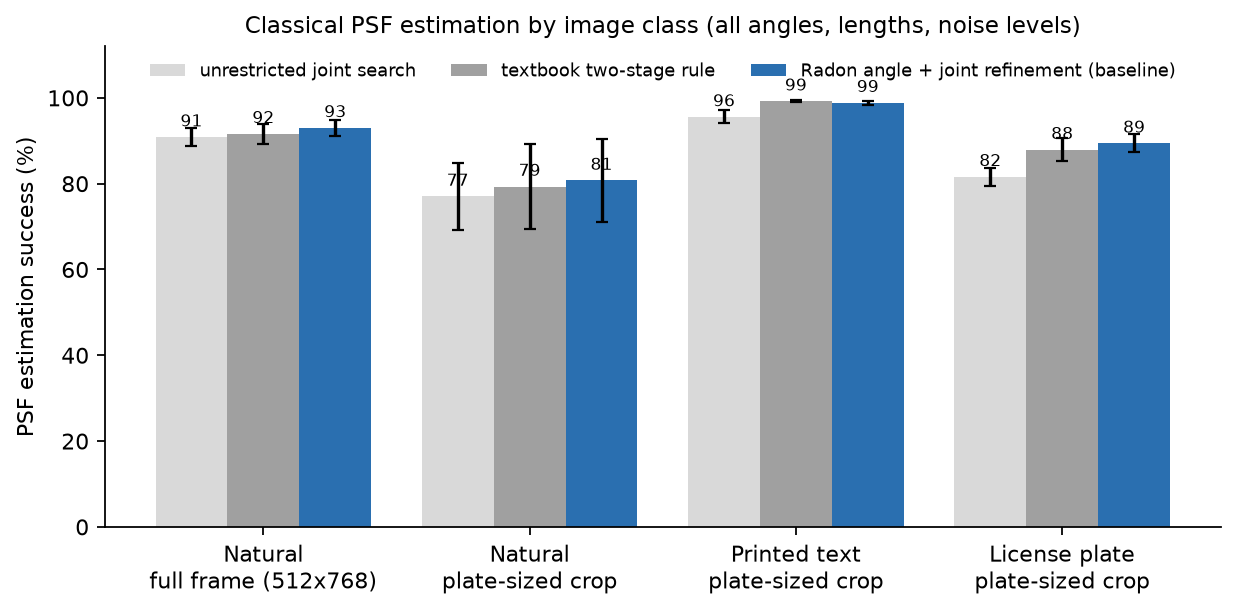
\includegraphics[width=0.66\textwidth]{02_success_by_class.png}
\caption{Estimation success on the test split (error bars: 95\% CI over source images). Three
angle strategies on identical trials; the baseline is the Radon-variance angle with a $\pm3^\circ$
joint refinement.}
\label{fig:sweepclass}
\end{figure}

\begin{table}[h]
\centering\small
\resizebox{\textwidth}{!}{\begin{tabular}{lcccc}
\toprule
 & natural, full frame & natural, crop & printed text, crop & plate, crop \\
\midrule
baseline (Radon angle + refinement) & \textbf{93.0} & \textbf{80.7} & 98.9 & \textbf{89.4} \\
textbook two-stage rule & 91.6 & 79.3 & \textbf{99.2} & 87.9 \\
unrestricted joint search & 90.9 & 77.0 & 95.6 & 81.6 \\
\midrule
baseline, $\sigma = 0.04$ & 80.3 & 60.6 & 96.2 & 75.6 \\
baseline, $L = 5$\,px & 71.3 & 56.1 & 94.9 & 58.1 \\
\midrule
PSNR blurred $\rightarrow$ restored (estimated PSF) & 24.6 $\rightarrow$ 25.3 & 23.2 $\rightarrow$ 23.5 & 15.6 $\rightarrow$ 17.7 & 20.3 $\rightarrow$ 22.7 \\
\quad restored with the true PSF (ceiling) & 26.0 & 24.7 & 17.8 & 23.6 \\
\quad restorations worse than the input & 6.3\% & 14.8\% & 0.7\% & 7.1\% \\
\bottomrule
\end{tabular}}
\caption{Success rate (\%) on the test split and restoration quality (RL with discrepancy stopping).}
\label{tab:sweep}
\end{table}

\begin{figure}[h]
\centering
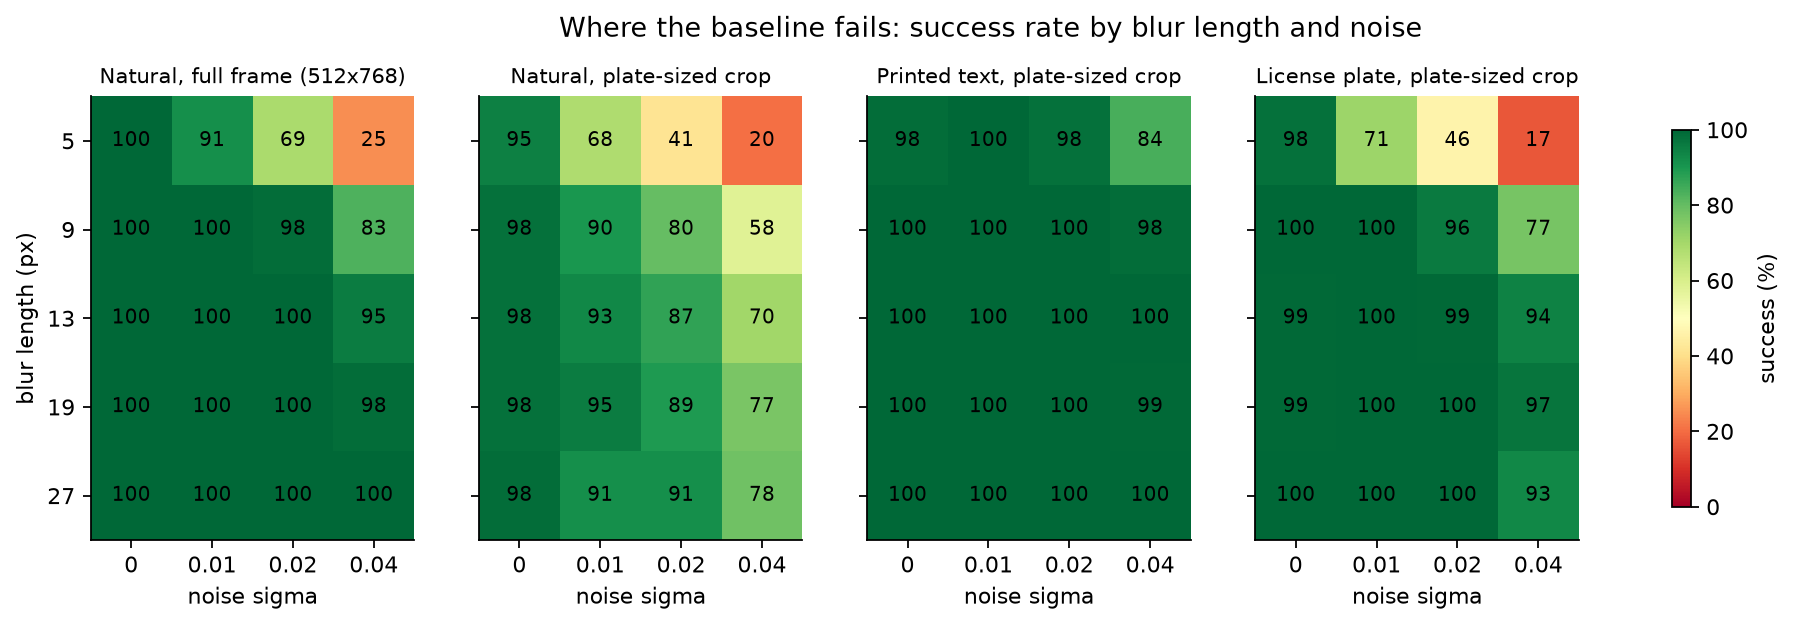
\includegraphics[width=\textwidth]{02_heatmap_length_noise.png}
\caption{Baseline success by blur length and noise level. The failure pocket is short blur under
noise, and it is much larger in a plate-sized window than at full frame.}
\label{fig:heat}
\end{figure}

\paragraph{Findings.} (i) The estimator is \emph{not} weaker on text content: printed text in a
plate-sized window is the easiest class (98.9\%), easier than natural texture in the same window
(80.7\%). Text is high-contrast and broadband, which is exactly what produces deep, regular sinc
nulls. (ii) What hurts is region size: the same Kodak images drop from 93.0\% at full frame to
80.7\% in the plate-sized window, because fewer samples carry the null pattern and the windowing
smears it. (iii) Within a window, the failures concentrate on short blurs under noise
(Fig.~\ref{fig:heat}): at $L=5$ the first null sits at $0.4$ of Nyquist, where noise dominates; at
$L\ge 13$ plates are above 94\% even at the highest noise level. (iv) Plates lie between text and
natural crops: the plate itself is high-contrast, but the window also holds bumper, grille and
background. (v) A wrong estimate is costly: in 7--15\% of the window trials the restoration with the
estimated PSF is worse than the blurred input, which is what the gate is for.

\paragraph{Angle strategy.} The Radon-variance angle is the more robust cue: the unrestricted joint
search, which phase~0 had favoured, has a 3--4$\times$ larger mean angle error (e.g.\ $7.1^\circ$ vs.\
$1.7^\circ$ on plates) because isolated deep dips in a wrong direction win the global minimum. The
$\pm3^\circ$ refinement around the Radon angle adds 1--2 points over the pure two-stage rule.

\subsection{O3: does pre-processing strengthen the blur signature?}
\label{sec:preproc}
Every candidate was inserted in front of the same estimator and run on the same test trials as
Section~\ref{sec:sweep} (8{,}960 trials per variant). Figure~\ref{fig:preproc} and
Table~\ref{tab:preproc} show the result.

\begin{figure}[h]
\centering
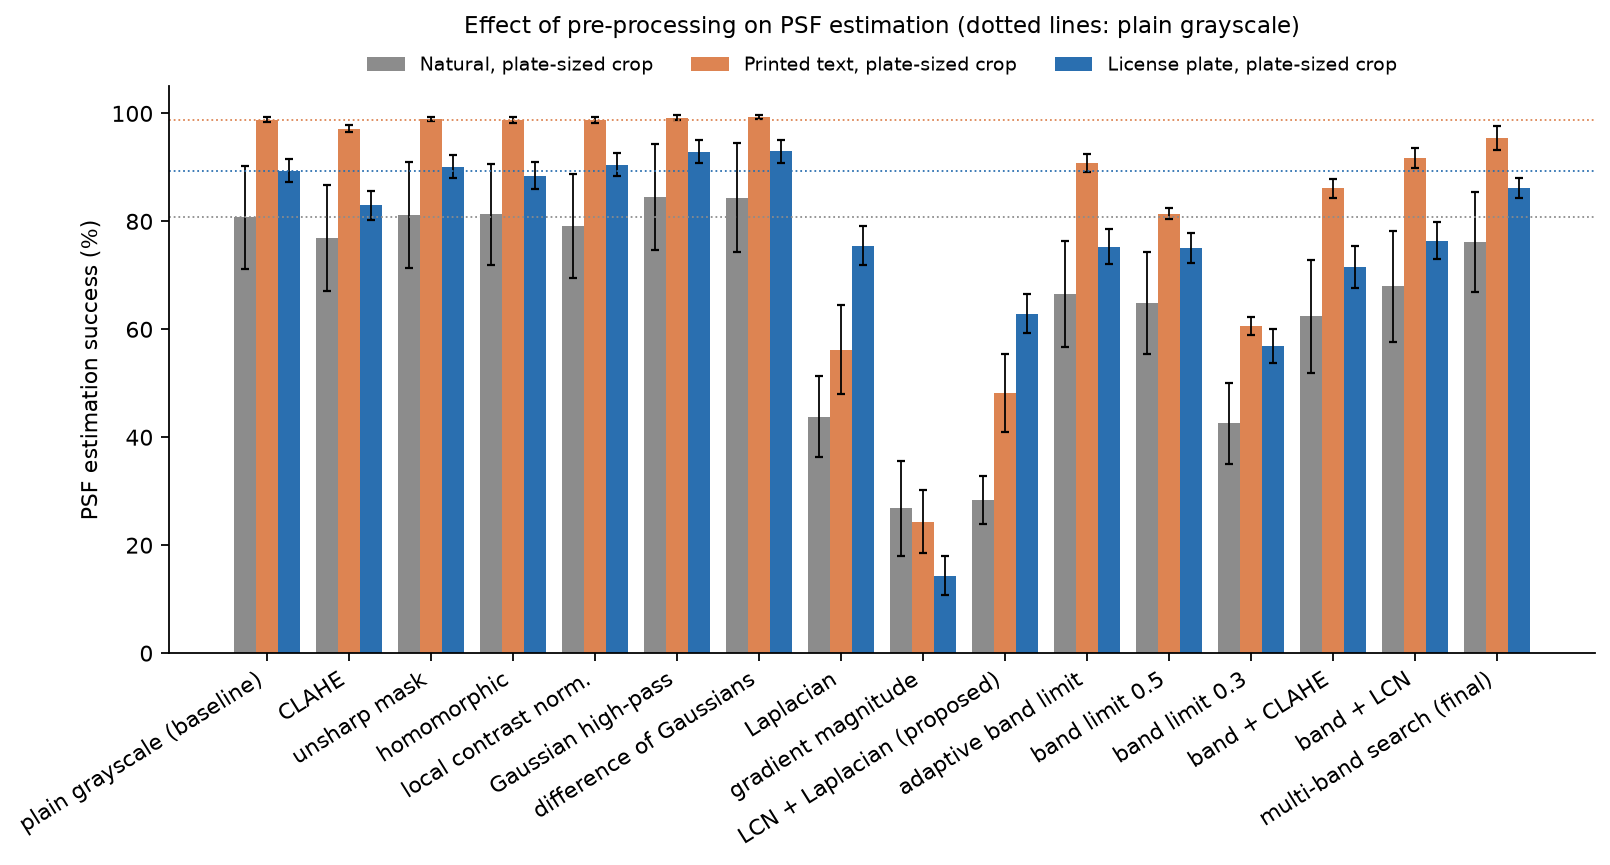
\includegraphics[width=\textwidth]{03_preprocess_success.png}
\caption{Estimation success per pre-processing variant (test split; dotted lines: plain grayscale).}
\label{fig:preproc}
\end{figure}

\begin{table}[h]
\centering\small
\begin{tabular}{lcccc|cc}
\toprule
variant & natural & text & plate & mean & plate, $L{=}5$ & plate, $\sigma{=}0.04$ \\
\midrule
plain grayscale (baseline) & 80.7 & 98.9 & 89.4 & 89.7 & 58 & 76 \\
CLAHE & 77.0 & 97.2 & 83.0 & 85.7 & 33 & 70 \\
unsharp mask & 81.2 & 99.0 & 90.1 & 90.1 & 61 & 76 \\
local contrast normalisation & 79.2 & 98.8 & 90.5 & 89.5 & 63 & 78 \\
Gaussian high-pass & \textbf{84.5} & 99.2 & \textbf{92.9} & \textbf{92.2} & \textbf{73} & \textbf{82} \\
difference of Gaussians & 84.4 & \textbf{99.3} & \textbf{92.9} & \textbf{92.2} & \textbf{73} & \textbf{82} \\
Laplacian & 43.8 & 56.2 & 75.5 & 58.5 & 62 & 22 \\
gradient magnitude & 26.8 & 24.4 & 14.3 & 21.8 & 20 & 9 \\
LCN + Laplacian (proposed) & 28.4 & 48.2 & 62.9 & 46.5 & 58 & 3 \\
adaptive band limit & 66.6 & 90.7 & 75.3 & 77.5 & 17 & 62 \\
band limit 0.3 & 42.6 & 60.6 & 57.0 & 53.4 & 0 & 54 \\
multi-band search (final) & 76.2 & 95.5 & 86.1 & 85.9 & 44 & 73 \\
\bottomrule
\end{tabular}
\caption{Estimation success (\%) on the synthetic test split. Homomorphic filtering and the band
limits combined with CLAHE/LCN are in \texttt{results/csv/03\_summary.csv}.}
\label{tab:preproc}
\end{table}

\paragraph{Findings.} The proposed stage --- local contrast normalisation followed by Laplacian edge
enhancement --- \emph{lowers} success from 89.7\% to 46.5\% and collapses under noise (3\% on
plates at $\sigma=0.04$). Strong derivative operators (Laplacian, gradient magnitude) behave the
same way: they multiply the spectrum by $|\omega|^2$ or worse, so the high-frequency noise floor
swamps the nulls and the operator's own structure adds spurious dips. Contrast normalisation alone
(CLAHE, LCN, homomorphic) is neutral to slightly harmful.

The one family that helps on synthetic data is the \emph{mild} band-pass: a Gaussian high-pass or
difference of Gaussians gains $+2.5$ points overall and $+15$ points on plates at $L=5$, the
failure pocket of Section~\ref{sec:sweep}. It flattens the strong low-frequency fall-off of the
spectrum without amplifying the noise band. These two operators were not part of the
development comparison on real plates (Section~\ref{sec:design}), so --- to avoid choosing on
test data --- they were not adopted; testing them on real plates is the most direct follow-up.

The final multi-band search costs 3.8 points here, all of it on short blurs ($L=5$: 44\% vs.\
58\% on plates), where the first null lies outside the lower bands and the full-band candidate
does not always win the directionality comparison. It was chosen for real plates, where it is
decisive (Section~\ref{sec:real}); on synthetic data, where noise is white and there is no
compression or resampling, the full spectrum carries real information up to Nyquist.

\subsection{O4: the confidence gate}
\label{sec:gateexp}
\paragraph{Labels.} A gate is judged by the restoration it guards. A case is \emph{helpful} if the
RL restoration with the estimated PSF is better than the input (PSNR on synthetic data, OCR
character accuracy on real plates) and \emph{harmful} if it is worse.

\paragraph{Signals.} Table~\ref{tab:auc} ranks the candidate signals by ROC AUC for predicting a
helpful restoration on the development sets. On synthetic data all four signals are strong
(AUC 0.91--0.97), with the proposal's dip depth the best. On real plates the picture changes:
on LPBlur dip depth and peak ratio remain informative (0.79--0.80), while on CCPD-Blur, where
only 4 of 150 restorations help at all, no single signal ranks well. The gate therefore needs a
test that targets the reason CCPD restorations fail --- the blur is not one uniform line --- which is
what split-half agreement checks.

\begin{table}[h]
\centering\small
\resizebox{\textwidth}{!}{\begin{tabular}{lcccc}
\toprule
dev set & dip depth & directional contrast & peak ratio & split-half agreement \\
\midrule
synthetic (all) & \textbf{0.97} & 0.91 & 0.94 & 0.93 \\
\quad plates & \textbf{1.00} & 0.93 & 0.99 & 0.97 \\
LPBlur & 0.79 & 0.64 & \textbf{0.80} & 0.60 \\
CCPD-Blur (4 helpful of 150) & 0.58 & 0.47 & 0.69 & 0.45 \\
\bottomrule
\end{tabular}}
\caption{ROC AUC of each gate signal for ``the restoration will help'' (text-aware estimator, dev data).}
\label{tab:auc}
\end{table}

\paragraph{Calibration.} A grid over the thresholds of dip depth, directional contrast and
agreement was scored on each development set by the \emph{net share} --- the net change the gate
lets through divided by the total change at stake, $\sum_{\text{accepted}} \Delta /
\sum |\Delta| \in [-1,1]$, so that refusing everything scores 0 and every harmful restoration is
charged at its full cost --- and the gate with the best mean over the three sets was frozen:
\[
  \text{accept} \iff \text{dip depth} \ge 4.4\,\sigma \;\wedge\; \ge 2 \text{ of the 4 image halves agree}.
\]
For comparison we also report the strictest operating point, which harms at most 5\% of the images
of every development set (dip depth $\ge 4.2\sigma$, directional contrast $\ge 4\sigma$, $\ge 3$
halves agree). Figure~\ref{fig:tradeoff} shows the full trade-off between harm avoided and helpful
restorations withheld.

\begin{figure}[h]
\centering
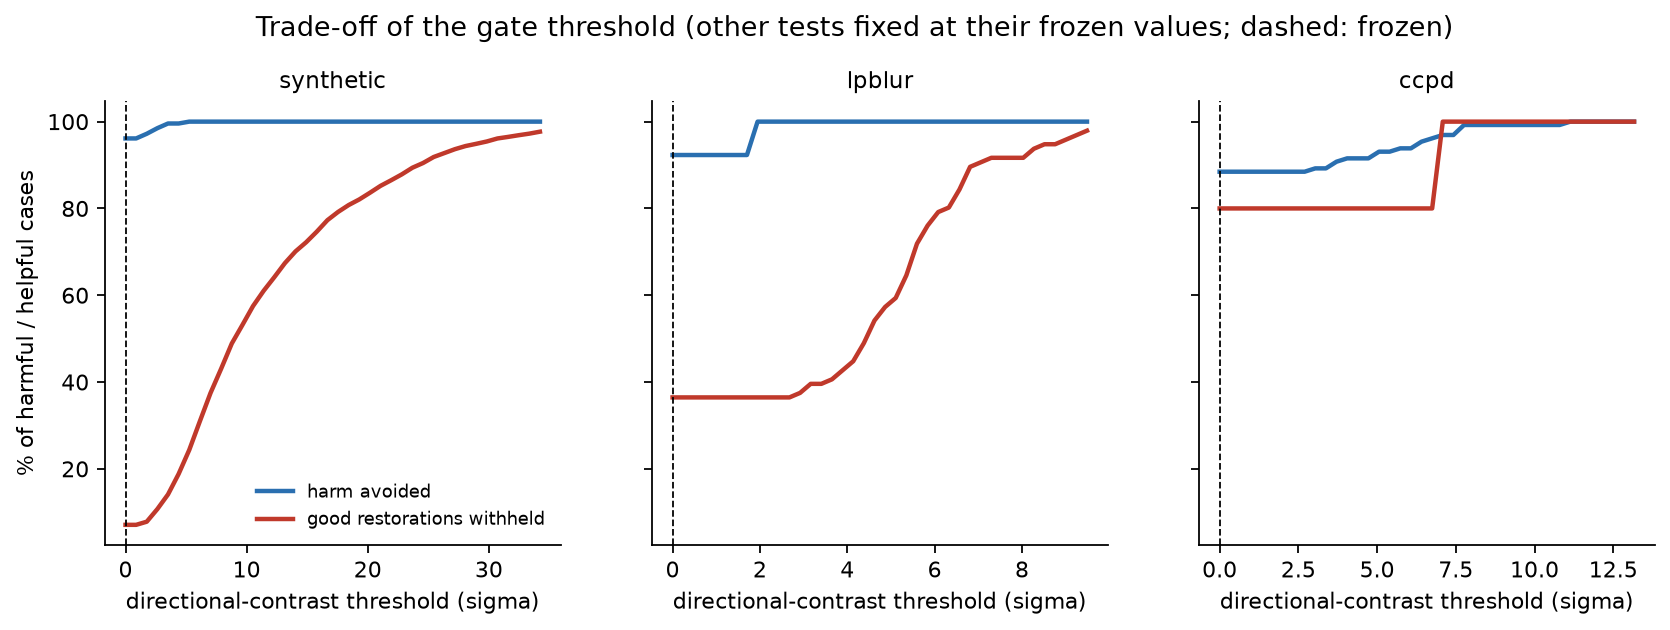
\includegraphics[width=\textwidth]{04_gate_tradeoff.png}
\caption{Harm avoided vs.\ helpful restorations withheld on the development sets, sweeping the
dip-depth threshold for each agreement requirement. CCPD-Blur has only four helpful cases, hence
the coarse steps.}
\label{fig:tradeoff}
\end{figure}

\paragraph{Held-out synthetic test.} Table~\ref{tab:gatetest} applies the frozen gate to the test
trials of Section~\ref{sec:preproc}. It refuses almost every harmful restoration (96--100\%) while
withholding 2--23\% of the helpful ones, and the share of images made worse falls from 4--20\% to
at most 0.4\%. Because the refused cases are exactly the ones with large losses, the mean PSNR gain
over all trials \emph{rises}, e.g.\ from $+1.5$ to $+3.0$\,dB on plates with the text-aware estimator.

\begin{table}[h]
\centering\small
\resizebox{\textwidth}{!}{\begin{tabular}{llcccccc}
\toprule
class & estimator & accepted & harm avoided & helpful withheld & images harmed & \multicolumn{2}{c}{mean gain (dB)} \\
 & & & & & (no gate $\rightarrow$ gate) & no gate & gate \\
\midrule
natural & baseline & 65\% & 99.7\% & 22\% & 14.8\% $\rightarrow$ 0.0\% & 0.24 & 1.25 \\
natural & text-aware & 60\% & 100\% & 23\% & 20.0\% $\rightarrow$ 0.0\% & $-0.31$ & 1.20 \\
text & baseline & 97\% & 100\% & 2\% & 0.7\% $\rightarrow$ 0.0\% & 2.14 & 2.19 \\
text & text-aware & 93\% & 100\% & 3\% & 4.1\% $\rightarrow$ 0.0\% & 1.74 & 2.12 \\
plate & baseline & 80\% & 96\% & 14\% & 7.0\% $\rightarrow$ 0.3\% & 2.34 & 3.06 \\
plate & text-aware & 78\% & 96\% & 13\% & 11.6\% $\rightarrow$ 0.4\% & 1.54 & 3.01 \\
\bottomrule
\end{tabular}}
\caption{The frozen gate on the held-out synthetic test split (2{,}560--3{,}840 trials per row).}
\label{tab:gatetest}
\end{table}

\subsection{O5: real blurred license plates}
\label{sec:real}
\paragraph{Protocol.} Held-out subsets of two public datasets, disjoint from the development subsets:
\textbf{LPBlur}~\cite{lpblur2024} (400 pairs drawn; 397 whose sharp image yields a six-character
reading, which serves as the reference text) --- real motion blur of moving vehicles with paired
sharp exposures --- and \textbf{CCPD-Blur}~\cite{ccpd2018} (400 street photographs with annotated
plate text; the plate region plus a margin is restored). Restoration is RL with 30 iterations. OCR
reads the rectified plate; on 200 sharp CCPD plates it reads 99.8\% of the characters correctly,
so it is not the bottleneck. 95\% confidence intervals are bootstrap intervals over images.

\begin{table}[h]
\centering\small
\begin{tabular}{l|ccccc|cccc}
\toprule
 & \multicolumn{5}{c|}{LPBlur ($n=397$)} & \multicolumn{4}{c}{CCPD-Blur ($n=400$)} \\
system & char.\ acc. & exact & worse & PSNR & SSIM & char.\ acc. & exact & worse & accepted \\
\midrule
blurred input & 0.176 & 3.3\% & -- & 21.62 & 0.642 & \textbf{0.759} & \textbf{42.2\%} & -- & -- \\
classical baseline & 0.241 & 7.1\% & 19.1\% & 20.09 & 0.581 & 0.237 & 5.5\% & 84.5\% & 100\% \\
baseline + gate & 0.188 & 4.8\% & 1.8\% & 21.56 & 0.640 & 0.652 & 35.2\% & 21.5\% & 29\% \\
text-aware, no gate & \textbf{0.497} & 25.4\% & 9.8\% & 21.08 & 0.657 & 0.185 & 3.8\% & 87.5\% & 100\% \\
text-aware + gate & 0.407 & 19.9\% & \textbf{0.8\%} & \textbf{21.95} & \textbf{0.682} & 0.684 & 37.0\% & 14.0\% & 18\% \\
text-aware + strict gate & 0.308 & 13.6\% & 0.3\% & 21.85 & 0.666 & 0.726 & 40.2\% & 5.5\% & 7\% \\
text-aware, Wiener & \textbf{0.497} & \textbf{26.7\%} & 9.3\% & 21.37 & 0.658 & 0.215 & 5.2\% & 85.2\% & 100\% \\
\bottomrule
\end{tabular}
\caption{Held-out real plates. \emph{char.\ acc.}: OCR character accuracy (95\% CIs: LPBlur
blurred 0.149--0.203, text-aware 0.459--0.536, text-aware + gate 0.366--0.447; CCPD blurred
0.730--0.786, text-aware + gate 0.652--0.718). \emph{exact}: whole plate read correctly.
\emph{worse}: images whose OCR accuracy drops. LPBlur accepted rates: baseline + gate 10\%,
text-aware + gate 43\%, strict 24\%.}
\label{tab:real}
\end{table}

\begin{figure}[h]
\centering
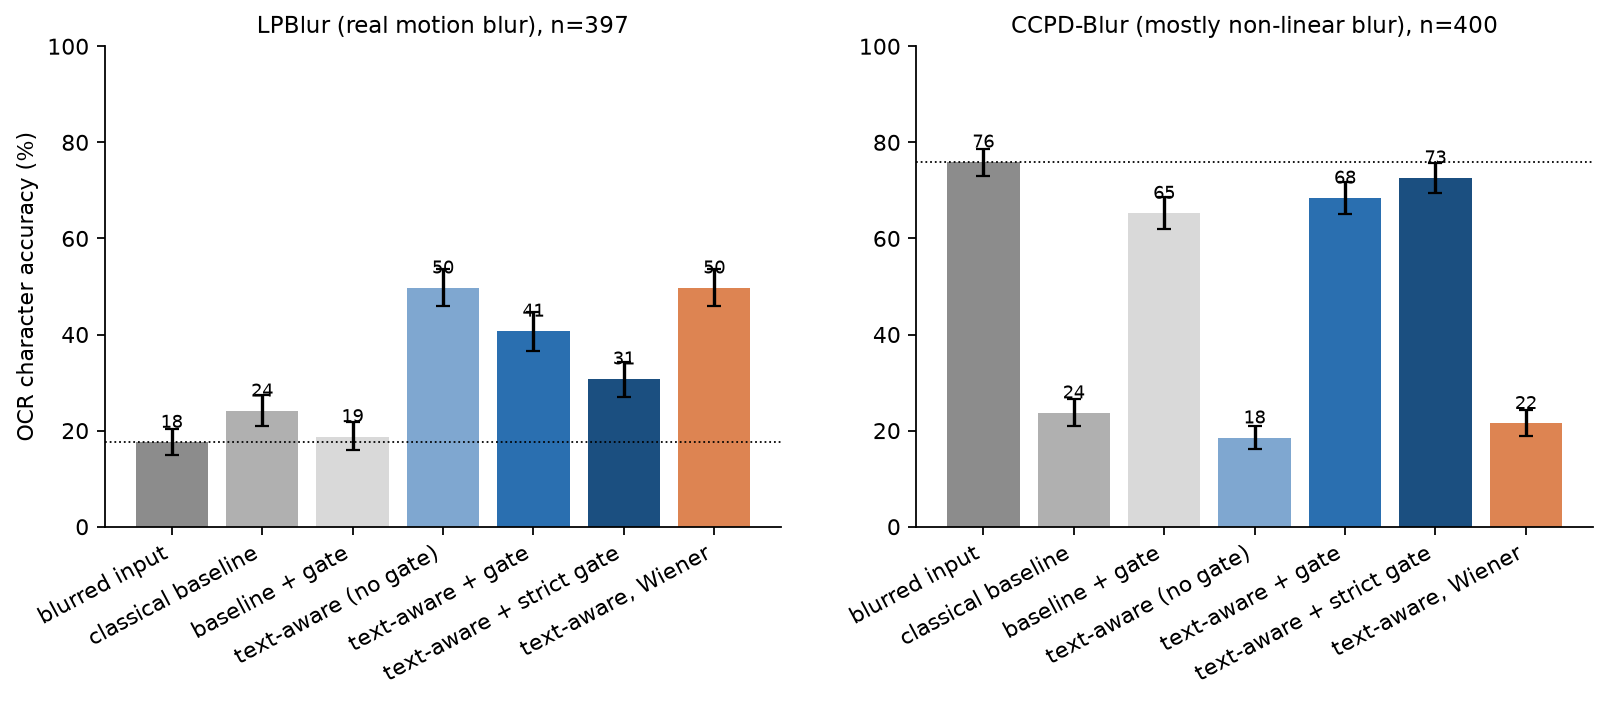
\includegraphics[width=\textwidth]{05_real_ocr.png}
\caption{OCR character accuracy on held-out real plates (dotted: blurred input).}
\label{fig:real}
\end{figure}

\paragraph{LPBlur: real motion blur.} The classical baseline lifts OCR accuracy only from 0.18 to
0.24 and makes 19\% of the plates worse; it also \emph{lowers} PSNR and SSIM. The text-aware estimator
reaches 0.50 --- almost three times the blurred input and twice the baseline --- and reads 25\% of
plates exactly, against 3\% blurred. The difference to the baseline lies entirely in the estimate
(both use the same RL), i.e.\ in the band limit (Section~\ref{sec:design}). With the gate, 43\% of the
plates are restored; only 0.8\% of all plates get worse, the mean accuracy is 0.41 (still $2.3\times$ the
input), and PSNR and SSIM are the best of all systems because no restoration with ringing gets
through. The gate withholds 96 restorations that would have helped, the price of refusing all but 3
of the 39 that would have hurt. Wiener with the same estimate performs on par with RL.

\paragraph{CCPD-Blur: mostly not linear motion.} Restoring every image with a line kernel is
destructive: accuracy falls from 0.76 to 0.19--0.24 and 85--88\% of the plates get worse --- the blur
in this set is predominantly defocus, mixed or non-uniform, which a straight line cannot explain,
and the plates are often already partly legible (42\% read exactly before restoration). The gate refuses 82\% of the images and recovers most of the loss
(0.68); the strict operating point refuses 93\% and comes within 3 points of the input (0.73). Neither
\emph{improves} on leaving CCPD-Blur alone, and we do not claim it does: the contribution of the
pipeline on this set is to recognise, for most images, that it should not act.

\begin{figure}[h]
\centering
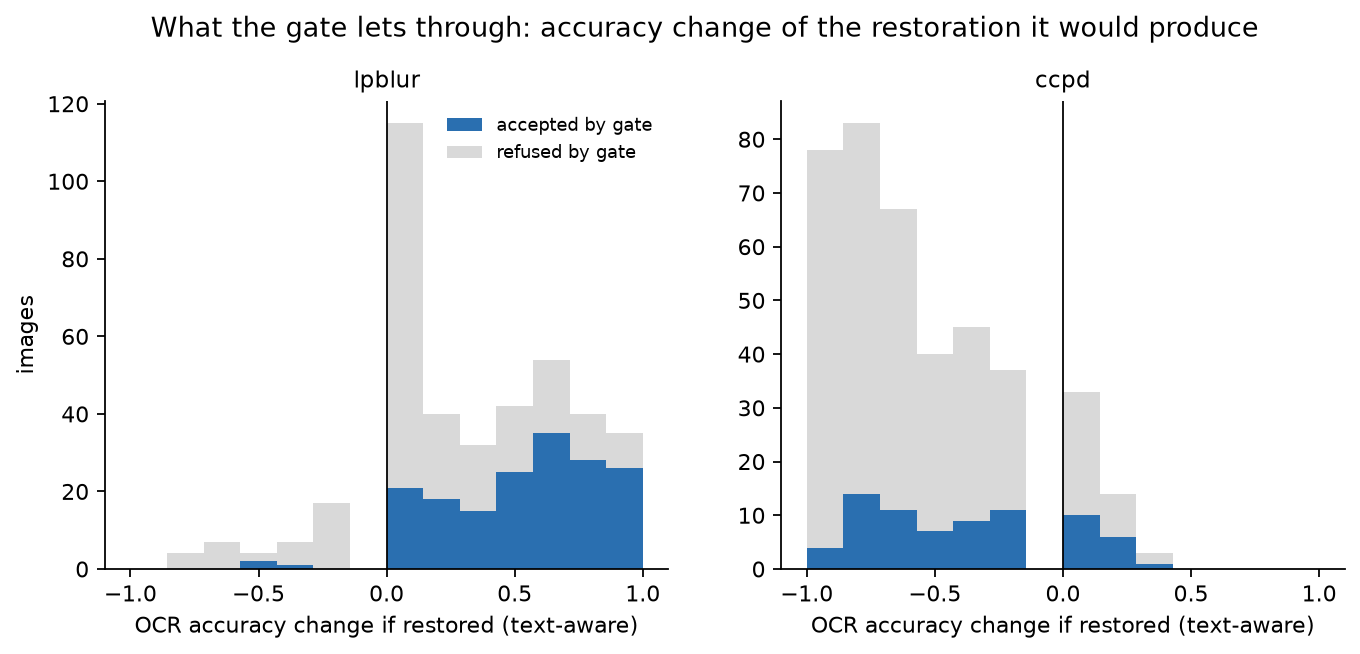
\includegraphics[width=0.9\textwidth]{05_gate_real.png}
\caption{Accuracy change the text-aware restoration would produce, split by the gate's decision.
On LPBlur the accepted cases are almost all improvements; on CCPD-Blur the gate refuses most
images, but a minority of the accepted ones still lose accuracy (the zero bin holds unchanged
readings).}
\label{fig:gatereal}
\end{figure}

\subsection{O1: the K\"ohler camera-shake benchmark}
\label{sec:kohler}
The benchmark~\cite{kohler2012} contains 48 photographs (4 scenes $\times$ 12 recorded hand-shake
trajectories replayed on a robot) with sharp frames along each trajectory. Reference kernels were
obtained by regularised Fourier division of each blurred image by a sharp frame; restoring with
them gives the ceiling. Ground truth for scenes 2 and 3 could not be retrieved in full (the archived
download is truncated), so PSNR is reported on the 24 images of scenes 1 and 4, following the
benchmark protocol (best PSNR over the sharp frames after intensity scaling and registration);
kernel comparisons use all 48 images.

\begin{figure}[h]
\centering
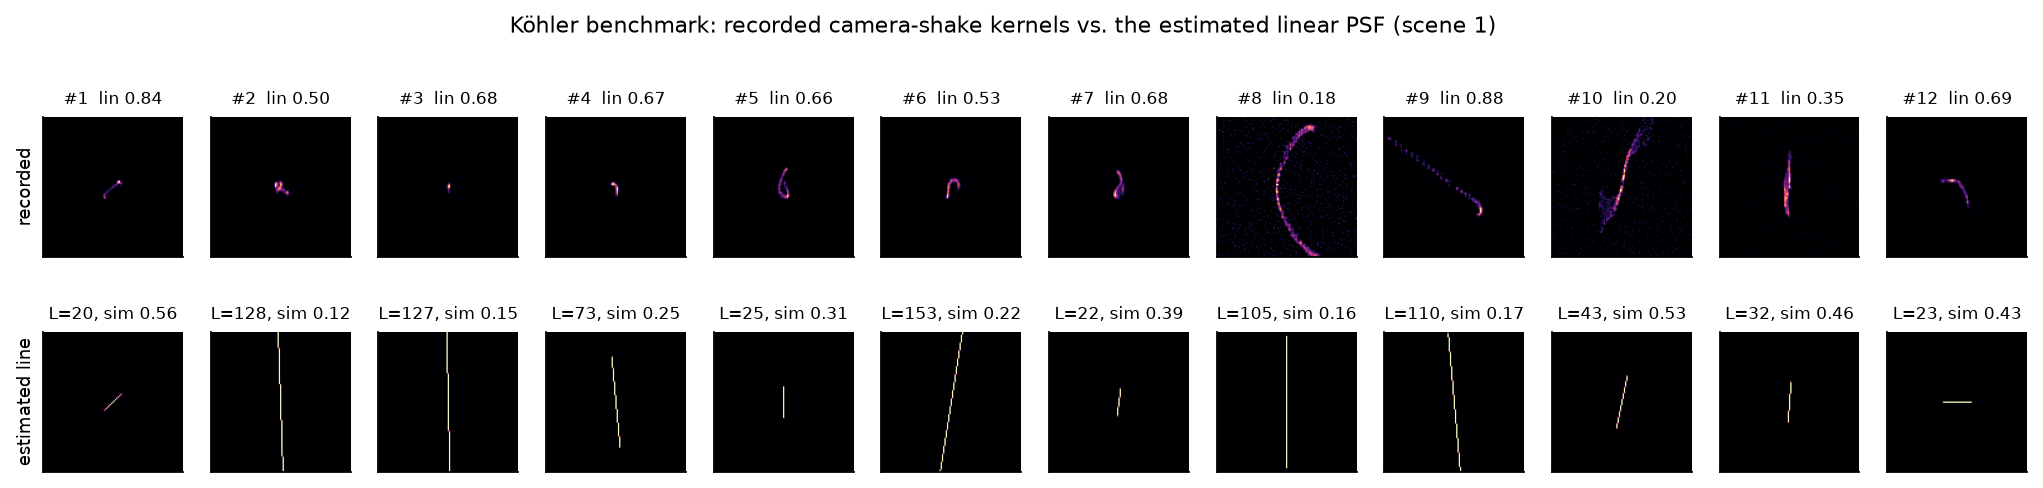
\includegraphics[width=\textwidth]{06_kohler_kernels.png}
\caption{Recorded camera-shake kernels (top, with a linearity score from second moments: 1 = straight
line) and the estimated line kernels (bottom; $L$ and cosine similarity to the recorded kernel).}
\label{fig:kohlerk}
\end{figure}

\begin{table}[h]
\centering\small
\begin{tabular}{lc}
\toprule
restoration (RL, 60 iterations, discrepancy stopping) & benchmark PSNR (dB), 24 images \\
\midrule
blurred input & 24.39 \\
recorded (reference) kernel --- ceiling & \textbf{29.24} \\
best straight-line fit to the recorded kernel & 23.42 \\
baseline estimate & 20.44 \\
text-aware estimate & 20.42 \\
text-aware estimate + gate (62\% accepted) & 24.08 \\
\bottomrule
\end{tabular}
\caption{K\"ohler benchmark.}
\label{tab:kohler}
\end{table}

\begin{figure}[h]
\centering
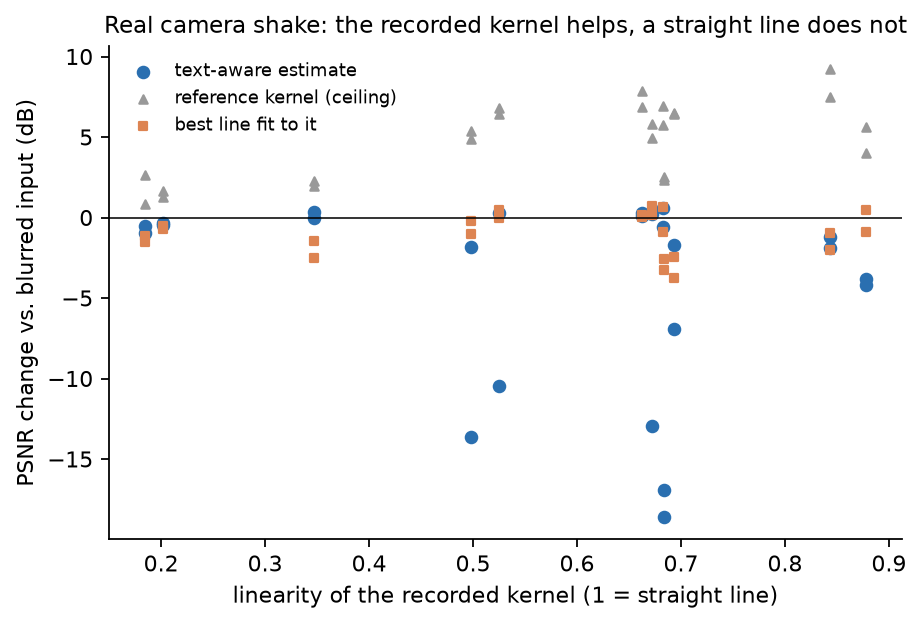
\includegraphics[width=0.6\textwidth]{06_kohler_gain_vs_linearity.png}
\caption{PSNR change against the blurred input versus how straight the recorded trajectory is.}
\label{fig:kohlerg}
\end{figure}

\paragraph{Findings.} Real hand shake is not a straight line (Fig.~\ref{fig:kohlerk}): only 2 of the
12 trajectories have a linearity above 0.75, and most are hooks and arcs. The consequence is
decisive: even the \emph{best} line kernel fitted to the recorded kernel loses 1\,dB against the
blurred input, while the recorded kernel gains 4.9\,dB. So the limiting factor on this benchmark is
the uniform-line model itself, which the proposal fixed as the scope, rather than the estimator. The
estimated lines are further off (75\% of restorations are worse than the input). On the two
near-linear trajectories the text-aware estimate finds the angle within $10^\circ$ in half the images,
against 38\% for the baseline. The gate helps less here than on plates: it accepts 15 of the 24
images and 9 of those restorations still hurt, because a curved trajectory still gives a strong,
consistent dominant direction in every image half. Detecting \emph{model} failure of this kind needs
a test of the line hypothesis itself (e.g.\ comparing the dip pattern with that of the fitted line),
which we leave as future work.

\subsection{Qualitative results}
\label{sec:gallery}
Figure~\ref{fig:worked} walks through the pipeline on one synthetic plate. Figures~\ref{fig:gallp}
and~\ref{fig:galcc} show held-out real plates. The rows are chosen by rule from the
experiment-5 results, not by hand: the largest accepted gains, typical accepted gains, the worst and
the best refused case, and the worst accepted case.

\begin{figure}[h]
\centering
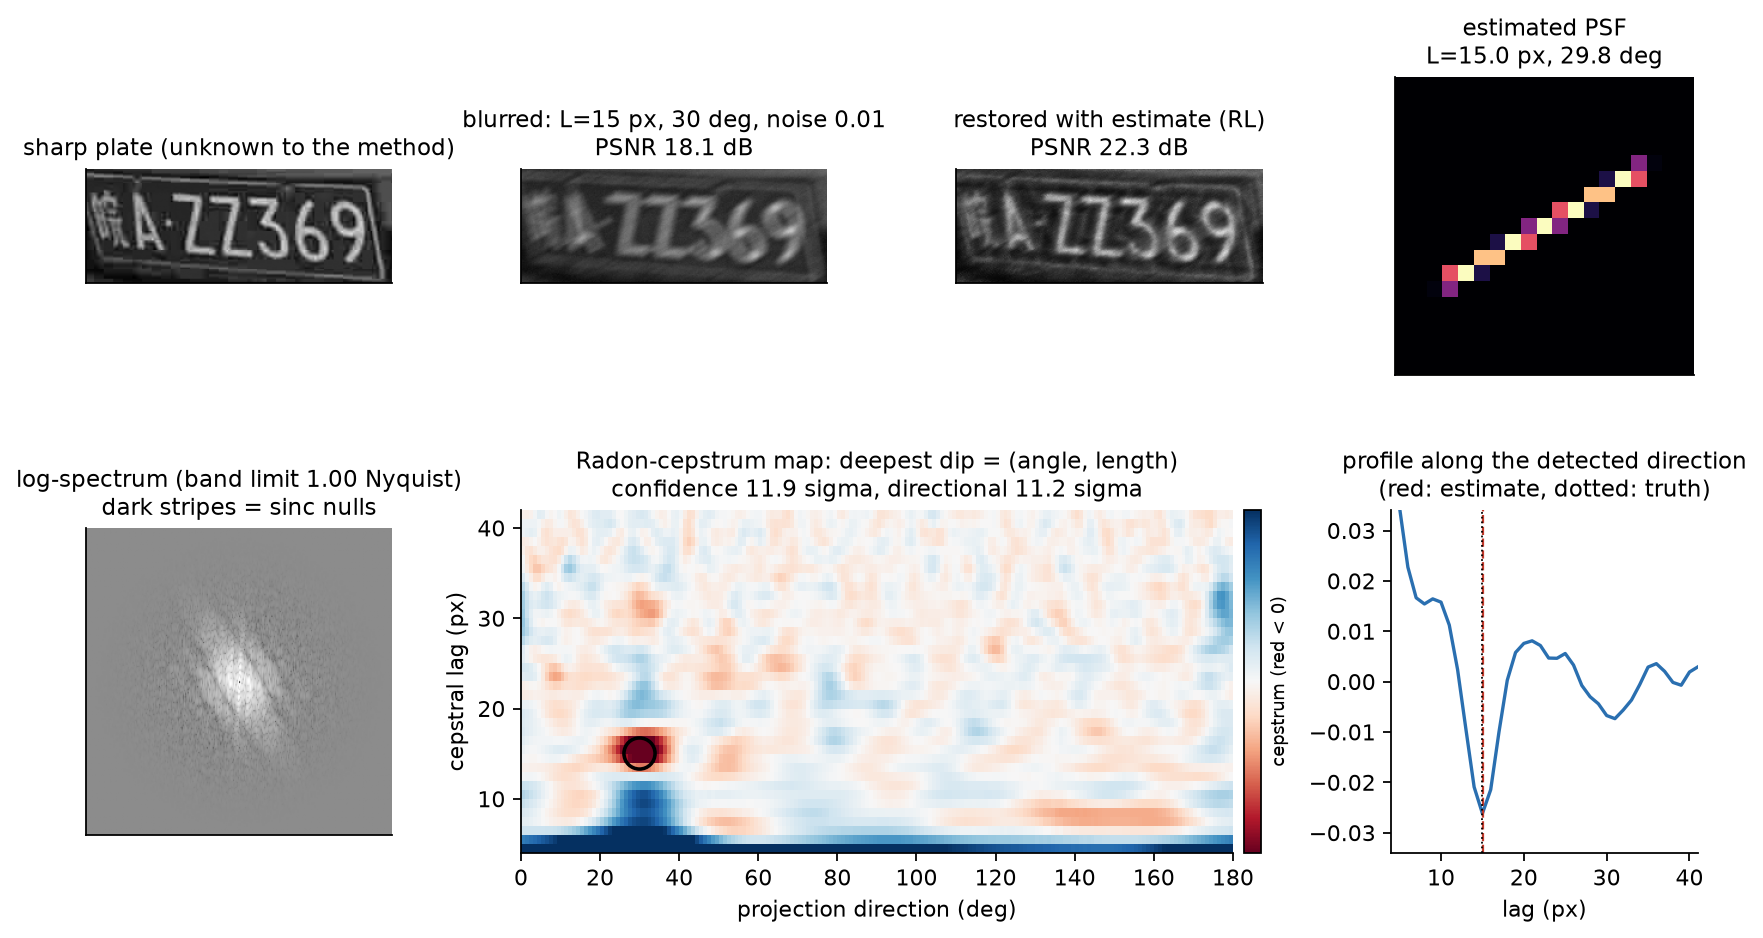
\includegraphics[width=\textwidth]{07_worked_example.png}
\caption{Worked example ($L=15$\,px, $30^\circ$, $\sigma=0.01$). The log-spectrum shows the dark
null stripes; the Radon--cepstrum map has a single deep dip at the true (angle, length); the
estimate is within $0.2^\circ$ and $0.1$\,px.}
\label{fig:worked}
\end{figure}

\begin{figure}[p]
\centering
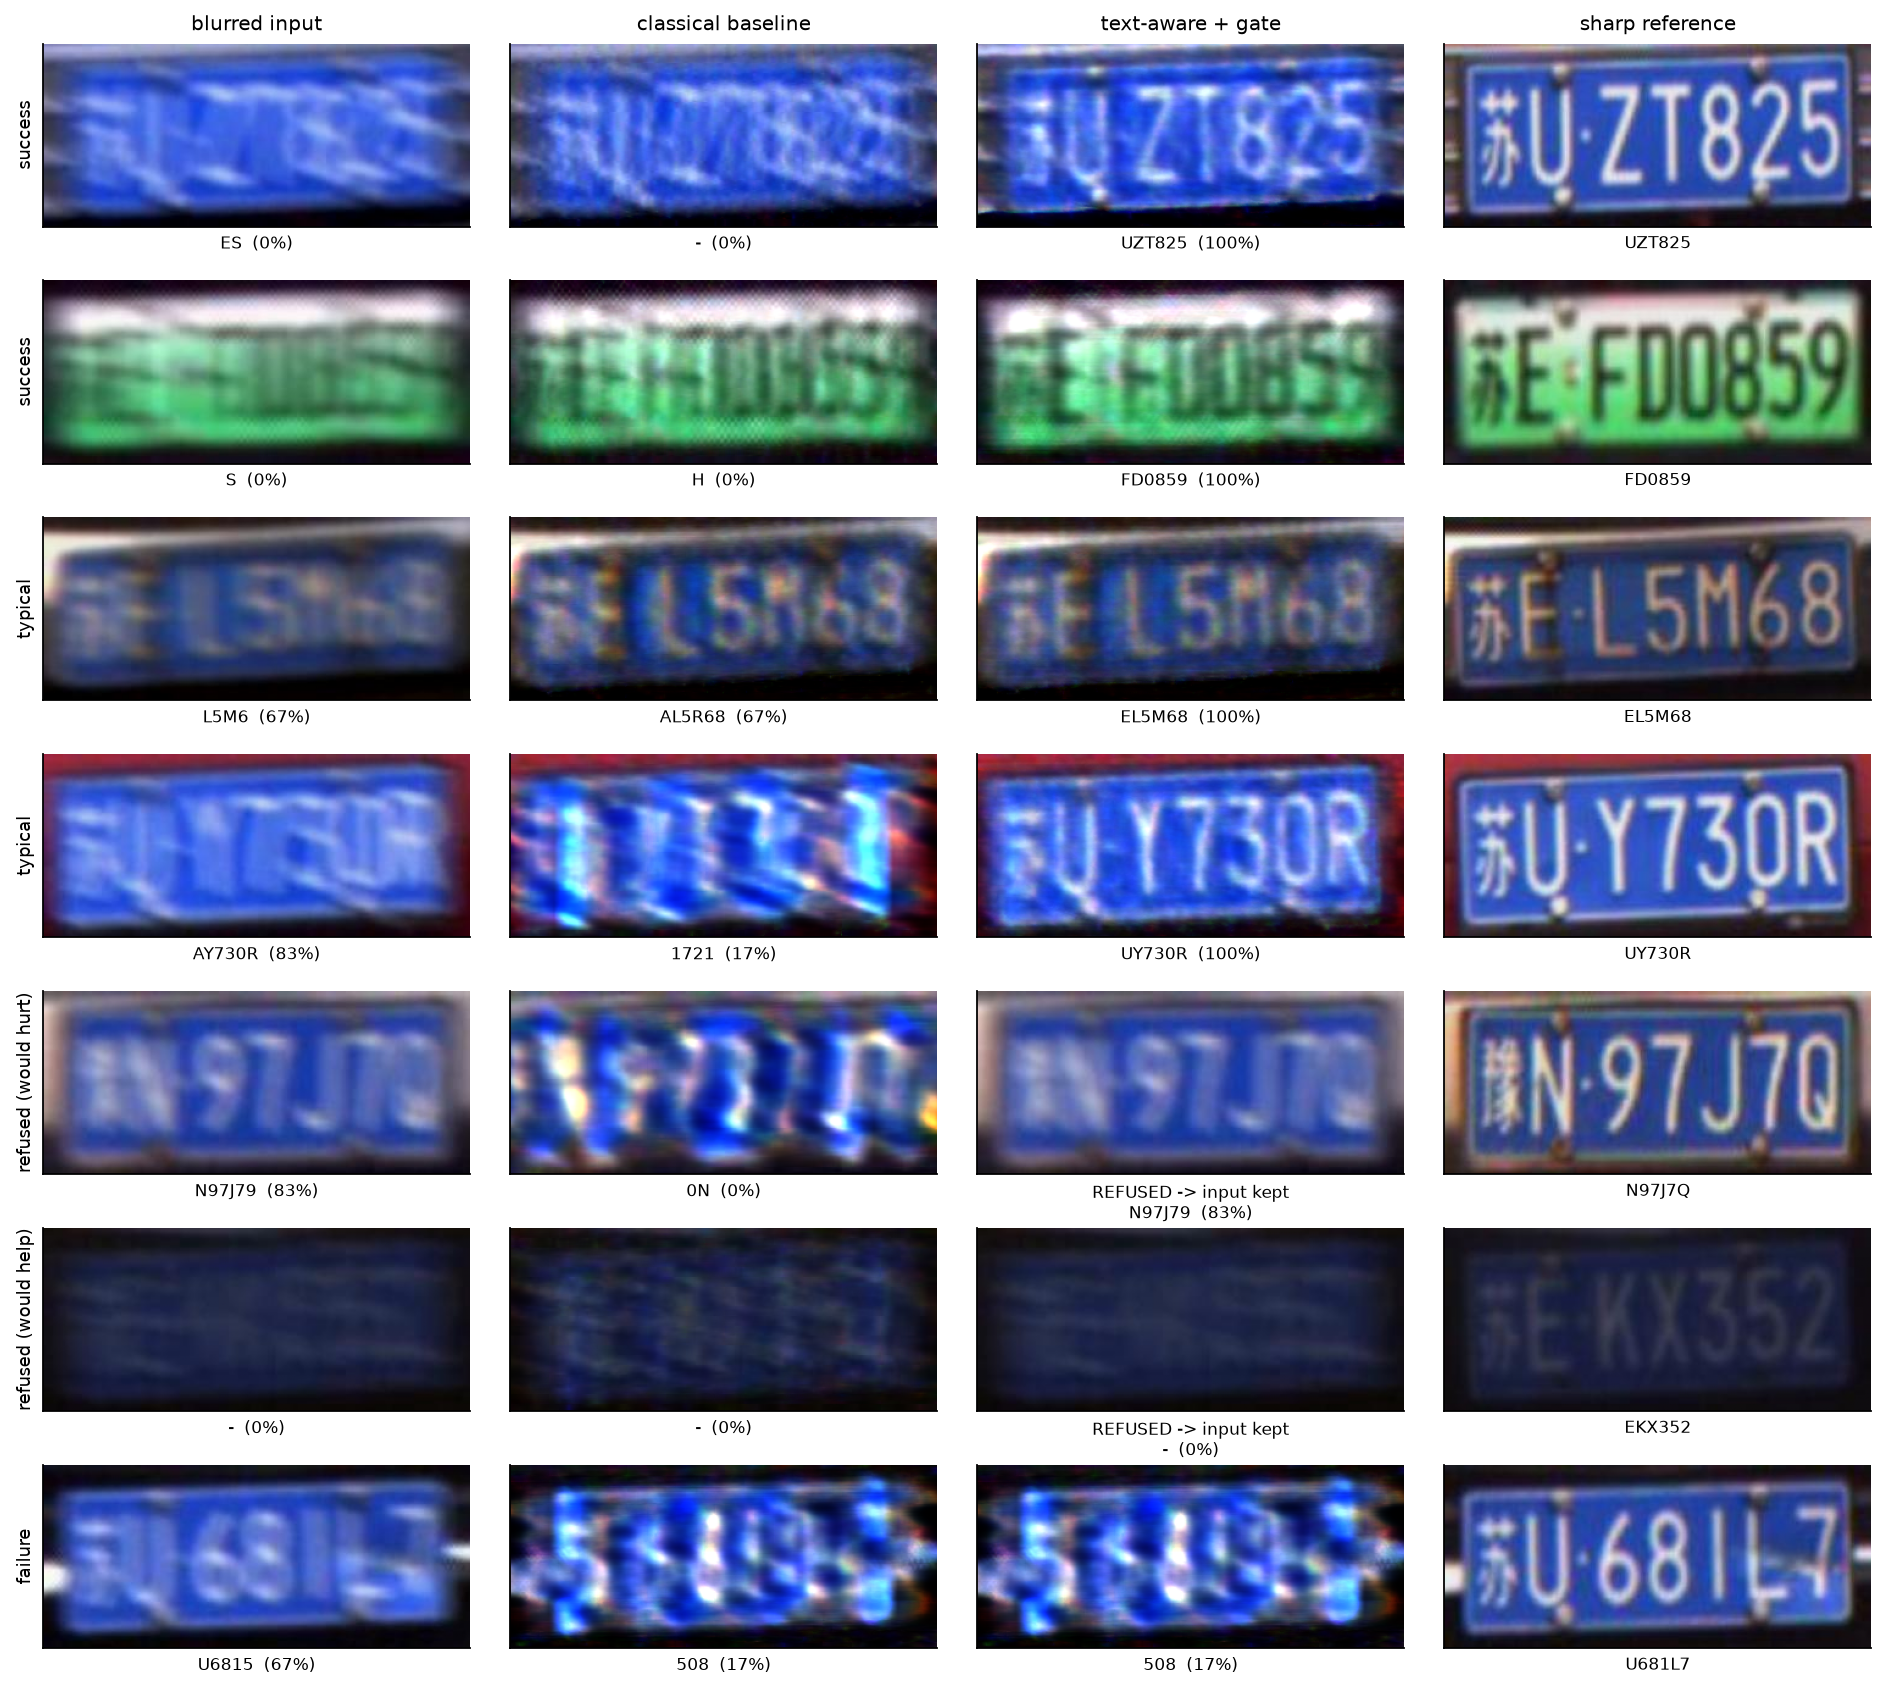
\includegraphics[width=0.93\textwidth]{07_gallery_lpblur.png}
\caption{LPBlur test plates (OCR reading and character accuracy under each image). The classical
baseline often produces strong ringing (rows 4--5): its full-band estimate is wrong. The gate refuses
a case that would have been destroyed (row 5) and, at the price of a missed improvement, a very dark
plate (row 6). Row 7 is a failure the gate let through.}
\label{fig:gallp}
\end{figure}

\begin{figure}[p]
\centering
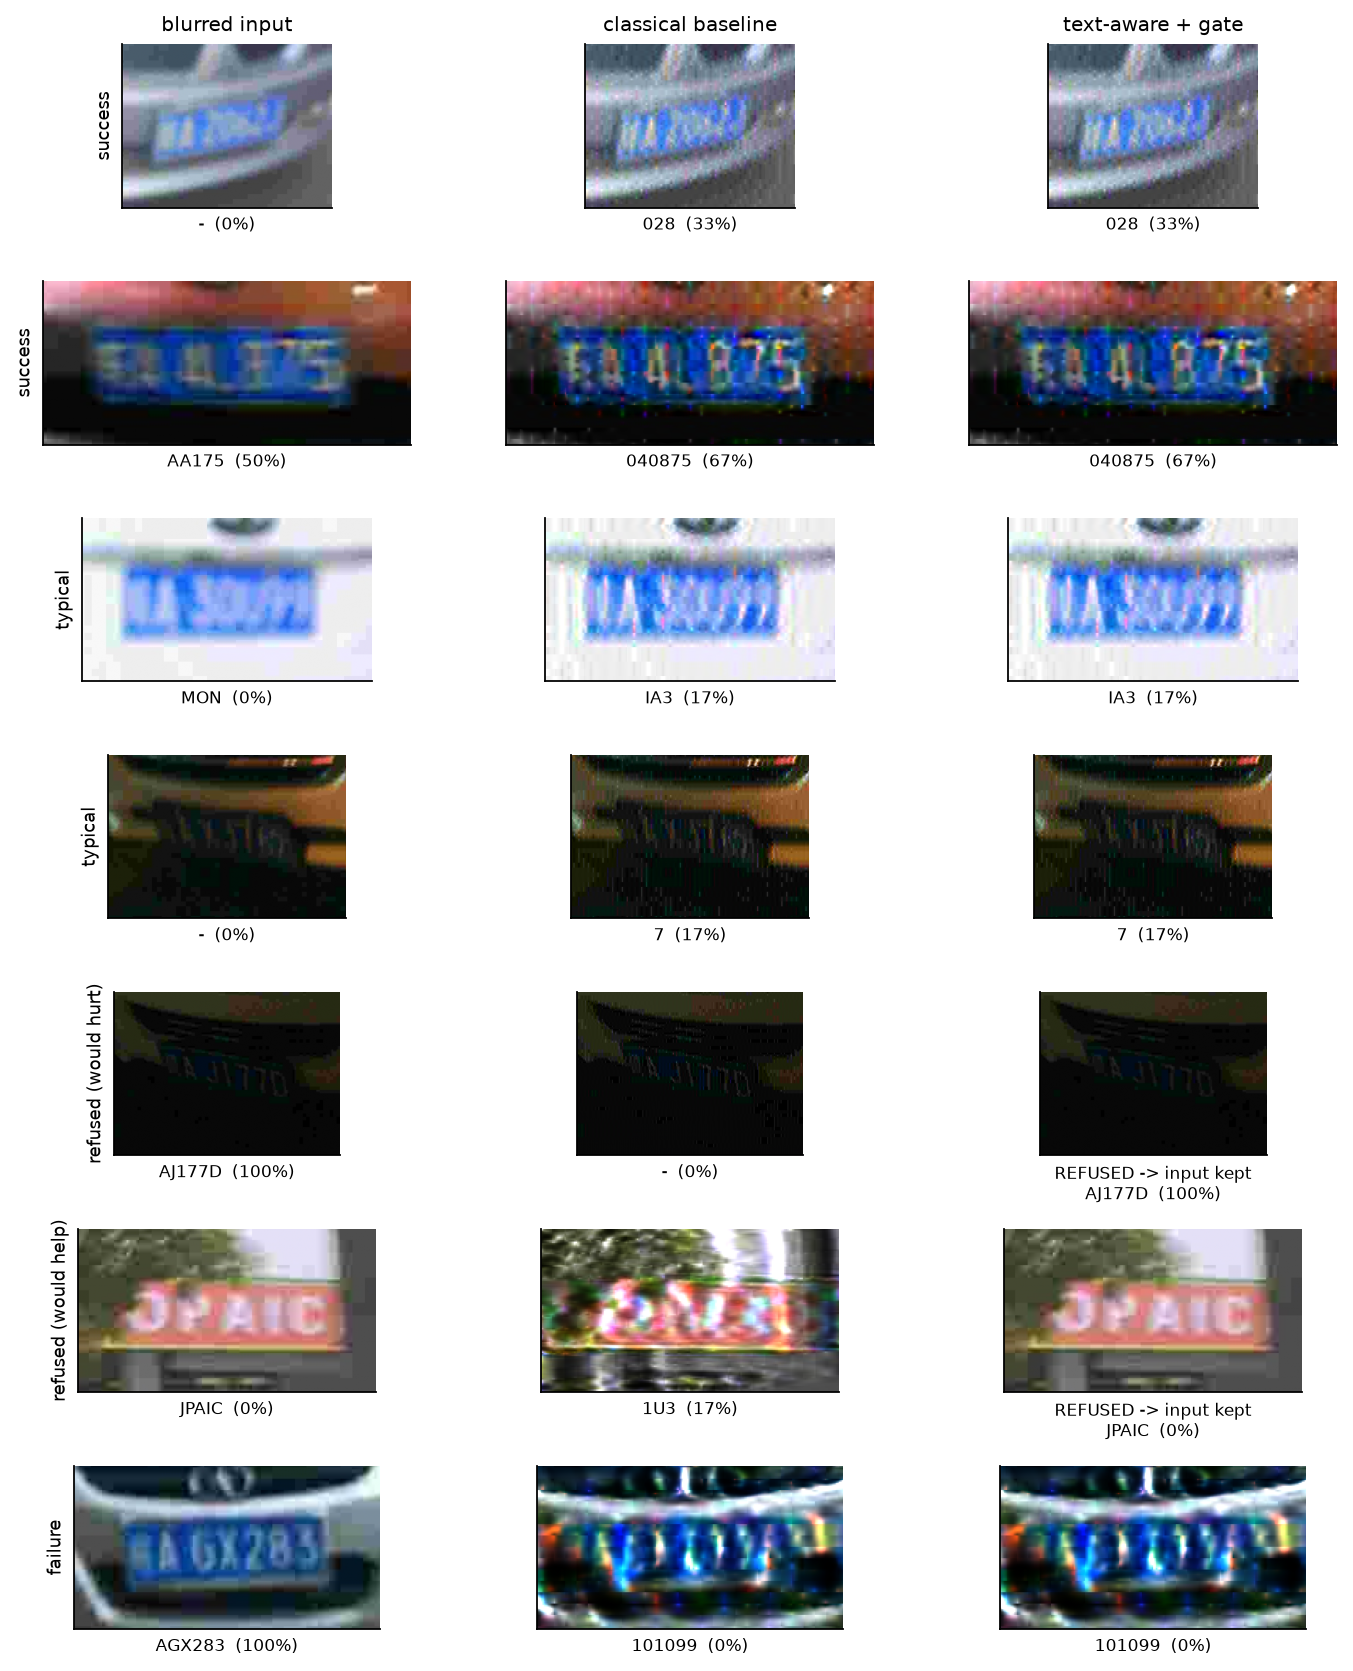
\includegraphics[width=0.93\textwidth]{07_gallery_ccpd.png}
\caption{CCPD-Blur test plates. Most of this blur is not linear motion; the few accepted restorations
help modestly, and the gate's refusals keep readable plates readable.}
\label{fig:galcc}
\end{figure}


% ================= DISCUSSION =================
\section{Discussion}
\label{sec:discussion}

\paragraph{What the hypothesis got right and wrong.} The proposal expected the classical estimator
to be weakest on text because sparse strokes give a weak blur signature. The controlled sweep
separates two effects the hypothesis had merged: \emph{content} and \emph{region size}. At full
frame, natural images are easy; cut to a plate-sized window they become the hardest class, while
printed text in the same window is the easiest --- its high-contrast, broadband strokes are exactly
what produces deep, regular nulls. Plates fall in between because the window also holds bumper and
background. What drives the failures is the number of samples that carry the null pattern (region
size), the noise level, and short blurs whose first null lies far out in the spectrum. Plates are
hard mainly because they are small.

\paragraph{Why edge enhancement fails and band limiting works.} The proposal's pre-processing idea
was to strengthen the strokes so the nulls stand out. In the frequency domain this is a high-pass
filter: it raises exactly the band where noise, JPEG blocking and resampling artefacts live and
where the sinc nulls are already the weakest, and it adds structure of its own. The blur
information of a long blur sits at low frequencies (its nulls are spaced $1/L$ apart), so the useful
operation is the opposite one --- discard the upper band. The multi-band search keeps the benefit
for short blurs by still trying the full band and letting the directionality of the dip decide.
The one edge-type operator that helped on synthetic data, a mild Gaussian high-pass, is consistent
with this picture: it flattens the steep low-frequency fall-off of the spectrum without boosting
the noise band, whereas the Laplacian multiplies the spectrum by $|\omega|^2$.

\paragraph{The gate is what makes the pipeline usable.} On real images the dominant risk is not a
slightly wrong kernel but a wrong \emph{model}: defocus, curved or non-uniform shake and compression
cannot be explained by one straight line, yet the estimator always returns one. Dip depth alone
cannot tell these cases apart. The test that does is physical: a uniform motion blur must give the
same estimate in every part of the region. This is cheap (four more estimates), needs no training
and has an interpretable refusal reason.

\paragraph{Limitations.}
\begin{itemize}
  \item One spatially uniform straight-line kernel per image (as scoped in the proposal). The
        K\"ohler results show how quickly this breaks on curved camera shake --- even the best line
        fit loses 1\,dB --- and the gate does not detect that failure, because a curved trajectory
        is still consistent across image halves.
  \item LPBlur has no text labels; the reference is OCR of the paired sharp image, so plates whose
        sharp image is misread are excluded, and the reader's own errors add noise.
  \item The gate is calibrated on a mixture of synthetic and real development data. Its thresholds
        reflect that mixture; a deployment with a very different blur distribution would need
        recalibration (the calibration script does this from labelled examples).
  \item The OCR read-out is a single off-the-shelf recogniser; absolute accuracies depend on it, the
        comparisons between systems much less so.
\end{itemize}

\paragraph{Future work.} Natural extensions within the classical toolbox are a two-segment or
curved kernel model with the same spectral evidence, local (patch-wise) estimation to handle
non-uniform shake, and using the split-half estimates not only to refuse but to detect where the
blur changes.


\bibliographystyle{plain}
\bibliography{references}

\appendix
% ================= APPENDIX =================
\section{Reproducibility}
\label{app:repro}

\paragraph{Code.} The library (\texttt{textdeblur/}) depends only on NumPy, SciPy, scikit-image,
OpenCV and pandas; RapidOCR is needed for the OCR read-out and Streamlit for the demo. The test
suite (\texttt{pytest}) checks, among other things, that the area-sampled PSF is an exact box on the
axes and sums to one, that the fast Radon transform matches \texttt{skimage.transform.radon}, that
the 1-D FFT of Radon projections equals the radial slice of the 2-D cepstrum (projection--slice
theorem), that the estimator recovers clean blurs over a grid of angles and lengths, that RL with the
true PSF improves PSNR, that a refused restoration returns the input bit-for-bit, and that every mode
of the demo runs.

\paragraph{Data splits.}
\begin{center}
\small
\resizebox{\textwidth}{!}{\begin{tabular}{lrrl}
\toprule
Source & dev & test & selection \\
\midrule
Kodak (natural) & 8 & 16 & kodim01--08 dev, 09--24 test \\
Rendered printed text & 8 & 16 & page index \\
Sharp CCPD-Base plates & 8 & 24 & stable hash of file name, CCPD blur score $\ge 60$, plate width 200--300\,px \\
LPBlur pairs & 150 & 400 & stable hash; test drawn from the remainder \\
CCPD-Blur & 150 & 400 & stable hash; test drawn from the remainder \\
K\"ohler & -- & 48 & all images (reference only, no tuning) \\
\bottomrule
\end{tabular}}
\end{center}
Synthetic trials: 8 angles ($0, 22, 45, 67, 90, 112, 135, 157^\circ$) $\times$ 5 lengths
(5, 9, 13, 19, 27\,px) $\times$ 4 noise levels ($\sigma = 0, 0.01, 0.02, 0.04$ on $[0,1]$, then 8-bit
quantisation) per source; the whole source is blurred before the $96\times256$ evaluation window is
cut, so content from outside the window is smeared into it as in a real photograph. A trial counts as
a success when the angle is within $5^\circ$ and the length within 2\,px.

\paragraph{Running.} \texttt{python experiments/run\_all.py} runs experiments 00--07 in order and writes
every table to \texttt{results/csv}, every figure to \texttt{results/figures} and every console
output to \texttt{results/logs}. Seeds are derived from the trial description, so reruns are
bit-identical. The full run takes about two to three hours on a 22-thread laptop.

\end{document}
